\documentclass[11pt]{beamer}
\usepackage[utf8]{inputenc}
\usepackage[T1]{fontenc}
\usepackage{lmodern}
\usepackage{tikz}
\usepackage{pgfplots}
\usepackage{graphicx}
\usepackage{geometry}
\usepackage{amsmath}
\usepackage{mathptmx}
\usepackage{physics}
\usepackage[siunitx]{circuitikz} 
\usepackage[percent]{overpic}

\pgfplotsset{compat=1.18}

\usetheme{Luebeck}
\usefonttheme[onlymath]{serif}

\usetikzlibrary{arrows.meta, positioning, shapes.multipart, fit}
\DeclareMathOperator*{\argmax}{arg\,max}
\newcommand{\mixer}[2]{  % #1 = reference coordinate, #2 = name
	\node[draw, thick, shape=circle, minimum size=24pt, at={#1}](#2){};
	\draw[rotate=45,line width=0.5pt] (#2.center)+(0,-12pt) -- +(0,12pt);
	\draw[rotate=-45,line width=0.5pt] (#2.center)+(0,-12pt) -- +(0,12pt);
}
\tikzset{block/.style = {draw, fill=white, rectangle,
		minimum height=3em, minimum width=2cm},
	input/.style = {coordinate},
	output/.style = {coordinate},
	pinstyle/.style = {pin edge={to-,t,black}},
	radiation/.style={decorate,decoration={expanding waves,angle=15,segment length=4pt}}
}

\setbeamerfont{footline}{size=\large}
\setbeamertemplate{page number in head/foot}[totalframenumber]

\begin{document}
	\author{Hamza FOUAD}
	\title[modulation CSS] {communication sans fil longue portée et basse consommation}
	\institute{Classes préparatoires aux grandes écoles}
	\date{Session 2025}

	\begin{frame}[plain]
		\maketitle
	\end{frame}

	\begin{frame}
		\frametitle{Plan de l'exposé :}
		\tableofcontents
	\end{frame}


	\section{Introduction}
	\begin{frame}
		\frametitle{Technologies selon portée et débit}
		
		\begin{center}
			\resizebox{0.95\linewidth}{!}{
				\rmfamily
				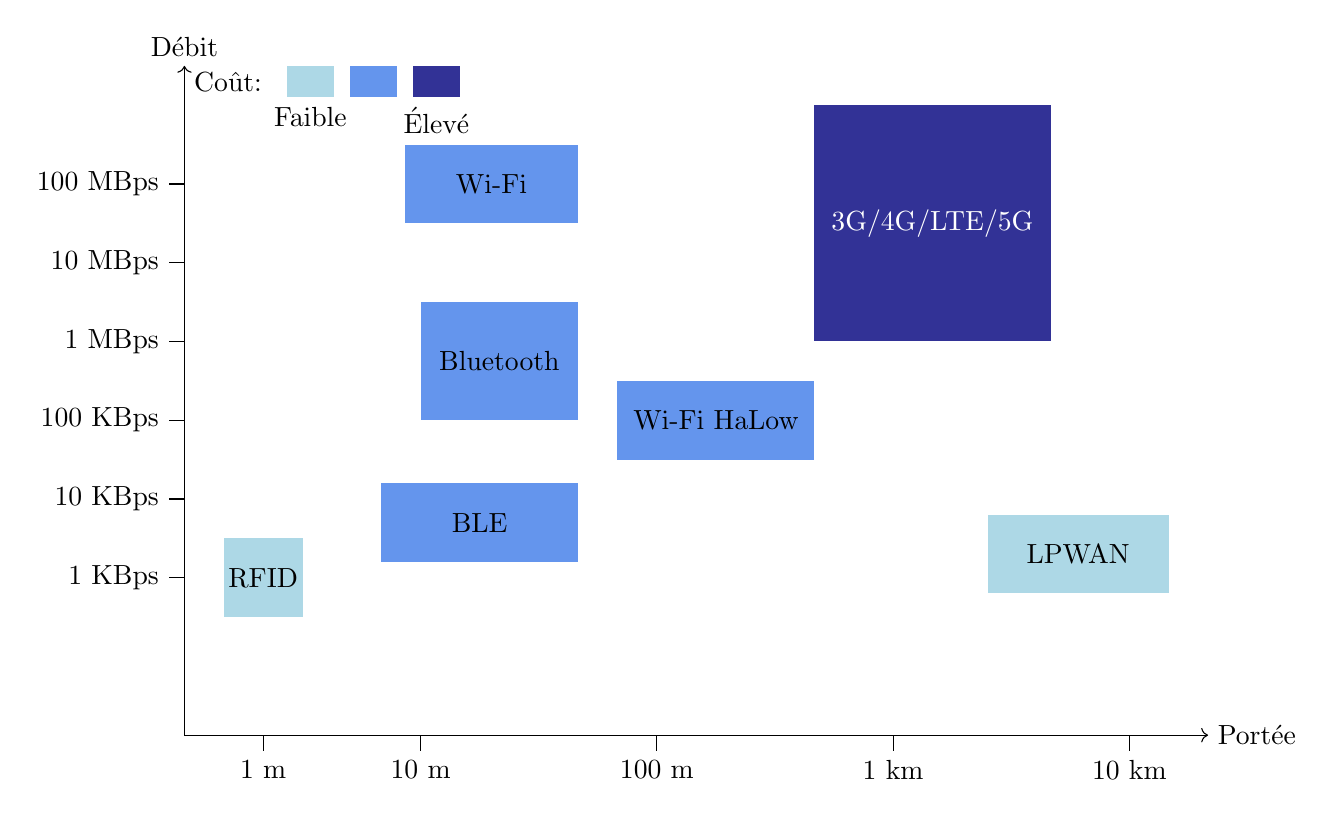
\begin{tikzpicture}
					% Define colors for cost levels
					\definecolor{costlow}{RGB}{173,216,230}    % Light blue
					\definecolor{costmedlow}{RGB}{100,149,237} % Medium light blue
					\definecolor{costmedhigh}{RGB}{70,130,180} % Medium blue
					\definecolor{costhigh}{RGB}{50,50,150}     % Dark blue
					
					% Axis
					\draw[->] (0,0) -- (13,0) node[anchor=west] {Portée};
					\draw[->] (0,0) -- (0,8.5) node[anchor=south] {Débit};
					
					% Y ticks
					\foreach \y/\label in {1/1 KBps,2/10 KBps,3/100 KBps,4/1 MBps,5/10 MBps,6/100 MBps}
					\draw (0,\y+1) -- (-0.2,\y+1) node[left] {\label};
					
					% X ticks
					\foreach \x/\label in {1/1 m,3/10 m,6/100 m,9/1 km,12/10 km}
					\draw (\x,0) -- (\x,-0.2) node[below] {\label};

					% Boxes for technologies
					\fill[costlow]     (0.5,1.5) rectangle (1.5,2.5) node[pos=.5, text=black] {RFID};
					\fill[costmedlow]  (3  ,4  ) rectangle (5,5.5) node[pos=.5, text=black] {Bluetooth};
					\fill[costmedlow]  (2.8,6.5) rectangle (5.0,7.5) node[pos=.5, text=black] {Wi-Fi};
					\fill[costmedlow]  (2.5,2.2) rectangle (5,3.2) node[pos=.5, text=black] {BLE};
					\fill[costmedlow]  (5.5,3.5) rectangle (8,4.5) node[pos=.5, text=black] {Wi-Fi HaLow};
					\fill[costhigh]    (8,5) rectangle (11,8) node[pos=.5, text=white] {3G/4G/LTE/5G};
					\fill[costlow]     (10.2,1.8) rectangle (12.5,2.8) node[pos=.5, text=black] {LPWAN};
					
					% Cost Legend
					\node at (0,8.3) [anchor=west] {Coût:};
					\fill[costlow]     (1.3,8.1) rectangle (1.9,8.5);
					\node at (1.6,8.1) [anchor=north] {Faible};
					
					\fill[costmedlow]  (2.1,8.1) rectangle (2.7,8.5);
					
					\fill[costhigh]    (2.9,8.1) rectangle (3.5,8.5);
					\node at (3.2,8.1) [anchor=north] {Élevé};
					
				\end{tikzpicture}
			}
		\end{center}
		
	\end{frame}
	
	\begin{frame}
		\frametitle{Technologies LPWAN existantes}
		\centering
		\includegraphics[width=0.8\linewidth]{frames/LPWANtech.png}
	\end{frame}
	
	\begin{frame}
		\frametitle{Problématique retenue}
		Comment modéliser la modulation CSS pour en analyser les performances et limitations théoriques, et concevoir un émetteur efficace, économe en énergie et robuste au bruit, adapté aux contraintes des réseaux IoT ?
	\end{frame}
	


	\section{Modélisation de la modulation CSS}
	\begin{frame}
		
		\frametitle{Quelques notations}
		
		\begin{columns}
			
			% Define B and b values
			\pgfmathsetmacro{\B}{5}
			\pgfmathsetmacro{\b}{1}
			
			\column{.4\textwidth}
			\begin{tikzpicture}
				\centering
				\begin{axis}[
					axis lines = middle,
					xlabel = $t$,
					ylabel = la frequence,
					ymin = 0, ymax = \B+2,
					xmin = 0, xmax = \B^2+5,
					restrict y to domain=0:4.99,
					samples = 1000,
					domain = 0:\B^2,
					width=5cm,
					height=4cm,
					xtick=\empty,
					ytick=\empty,
					extra y ticks={0, \B},
					extra y tick labels={$f_{min}$, $f_{max}$},
					extra y tick style={
						tick label style={anchor=east}
					},
					extra x ticks={20 ,\B^2},
					extra x tick labels={$t_f$, $T$},
					extra x tick style={
						tick label style={anchor=north}
					},
					]
					\addplot[
					blue,
					thick,
					] {mod(x/\B + \b, \B)};
					\draw[dashed] (0,1) -- (25,1);
					\draw[<->] (8,0) -- (8,5) node[midway,right] {$B$};
					\draw[<->] (1,0) -- (1,\b) node[midway,right] {$b$};
					\draw[dashed] (0,5) -- (25,5);
				\end{axis}
			\end{tikzpicture}
			
			
			\column{.5\textwidth}
			$f_s(t)$ est la fonction de fréquence.\\
			$s$ est le mot binaire à transmettre, composé de $SF$ bits
			$\displaystyle s = \sum_{i=0}^{SF-1} s_i 2^i$; $s_i \in \{0,1\}$;\\
			$SF$ est le facteur d'étalement (Spread Factor).\\
			On fixe la période $T = \dfrac{2^{SF}}{B}$\\
		\end{columns}
	\end{frame}
	
	\begin{frame}
		
		\begin{columns}
			
			% Define B and b values
			\pgfmathsetmacro{\B}{5}
			\pgfmathsetmacro{\b}{1}
			
			\column{.4\textwidth}
			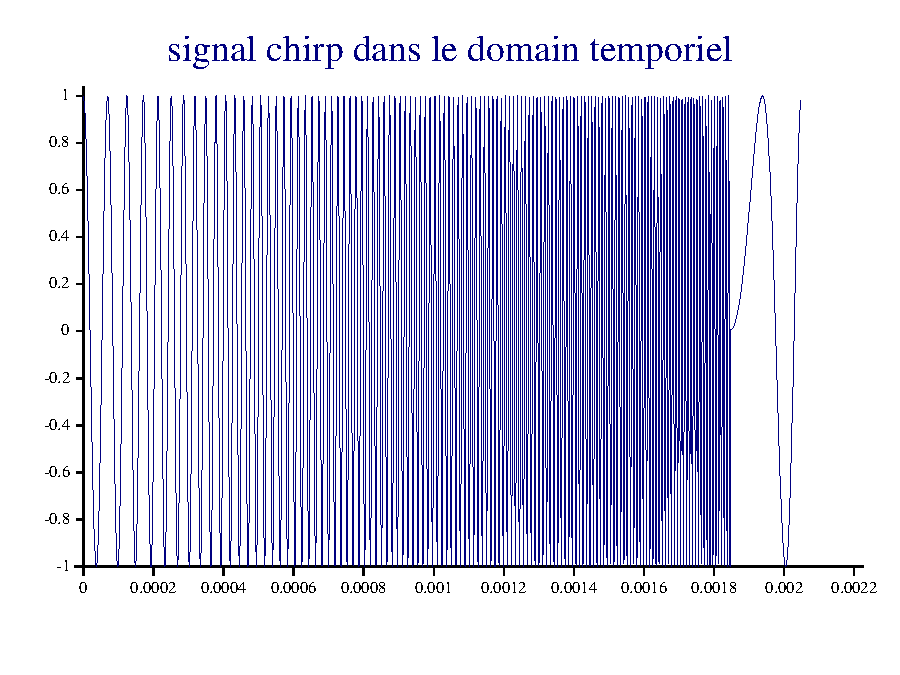
\includegraphics[width=1.1\textwidth, height=5cm]{frames/c_s.pdf}
			
			
			\column{.6\textwidth}
			$f_s(t) = (at + b)_{\bmod B}$\\
			$\displaystyle a = \dfrac{df_s(t)}{dt} = \dfrac{B}{T}$ ;
			$b_s = \dfrac{s}{2^{SF}} B$\\
			$\Rightarrow f_s(t) = (s + \dfrac{t}{T}2^{SF})_{mod  2^{SF}} \dfrac{B}{2^{SF}}$\\~\\
			$\displaystyle \varphi(t) \equiv \int\omega dt \equiv 2\pi \int_{0}^{t}\varDelta f_s(\tau) d\tau$\\
			Modulation à phase continue, sans discontinuité de phase :\\$\varphi(T) \equiv \varphi(0) \equiv 0$ $mod$ $2\pi$\\
		\end{columns}
		\centering
		L'expression du signal est : $\displaystyle c_s(t) = e^{j\varphi(t)}$
		\begin{align*}
			c_s(t) = \begin{cases} \exp ({j 2 \pi ({ ({\frac {s}{2^{SF}}}) Bt + \frac {B}{2T} t^{2}}) }), & 0 \leq t < t_f \\
				\exp ({j 2 \pi ({ ({\frac {s}{2^{SF}} - 1}) Bt + \frac {B}{2T} t^{2} }) }), & t_f \leq t < T \end{cases}
		\end{align*}
	\end{frame}
	
	\begin{frame}
		Voici un exemple d’un signal composé de 4 symboles avec un facteur d’étalement $SF = 2$, chaque symbole est composée de $SF = 2$ bits.\\
		\includegraphics[width=\textwidth]{frames/CSSword.png}
		Les signaux correspondant à chaque symbole pour un $SF$ donné sont orthogonaux (voir annexe)\\
	\end{frame}
	
	\begin{frame}
		\frametitle{Modélisation du bruit}
		on peut modeliser le bruit réel par le bruit blanc gaussien additif.\\~\\~\\
		\centering
		\includegraphics[width=\linewidth]{frames/awgn.png}
	\end{frame}
	
	\begin{frame}
		On peut quantifier l’effet du bruit par: $\displaystyle SNR = 10\log_{10}(\frac{P_s}{P_b})$
		\begin{columns}
			\column{0.4\textwidth}
			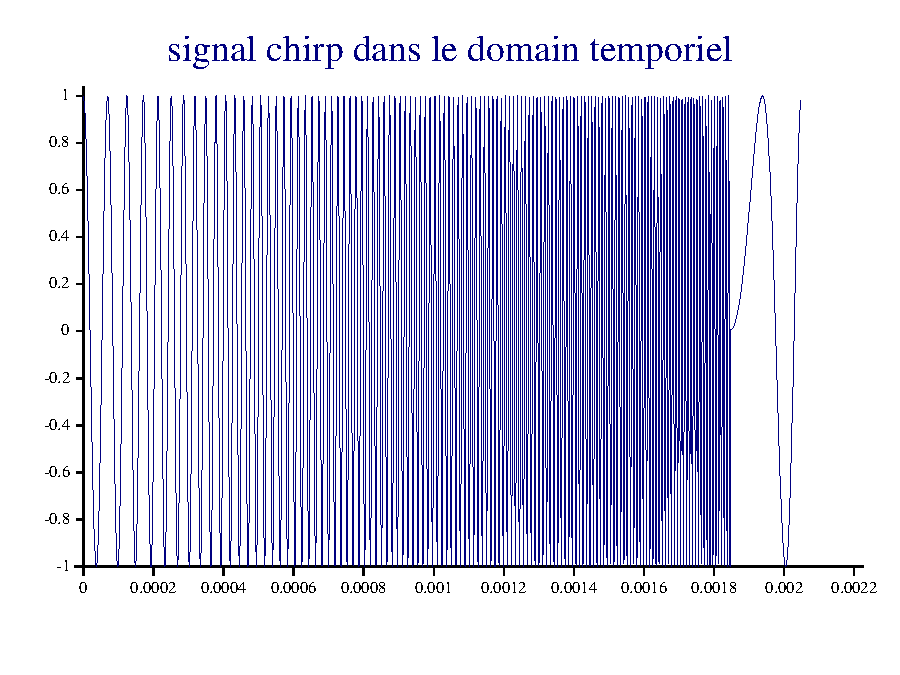
\includegraphics[width=\linewidth]{frames/c_s.pdf}
			\column{0.4\textwidth}
			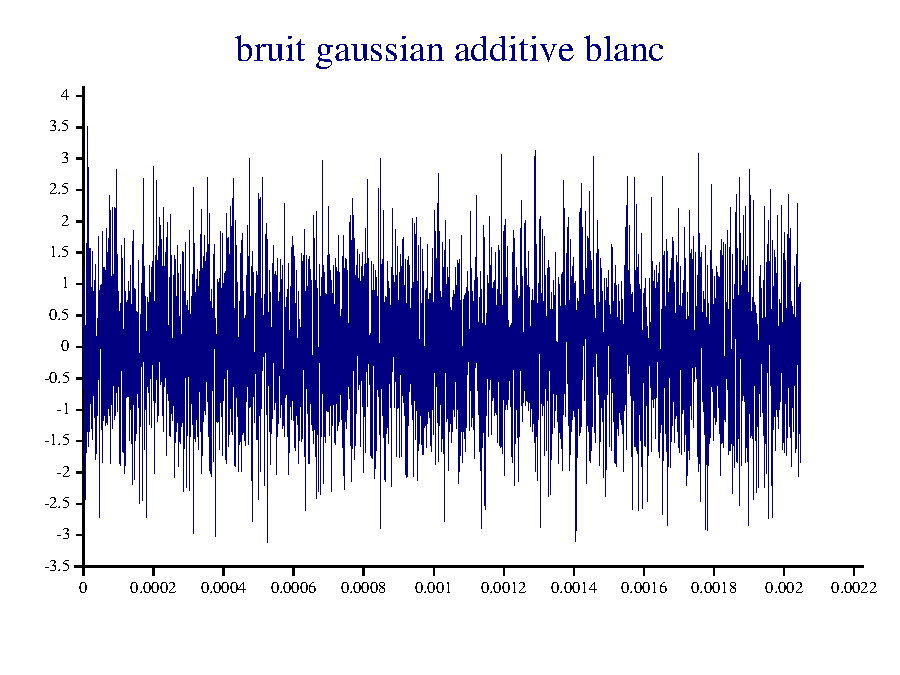
\includegraphics[width=\linewidth]{frames/noise.pdf}
			\column{0.4\textwidth}
			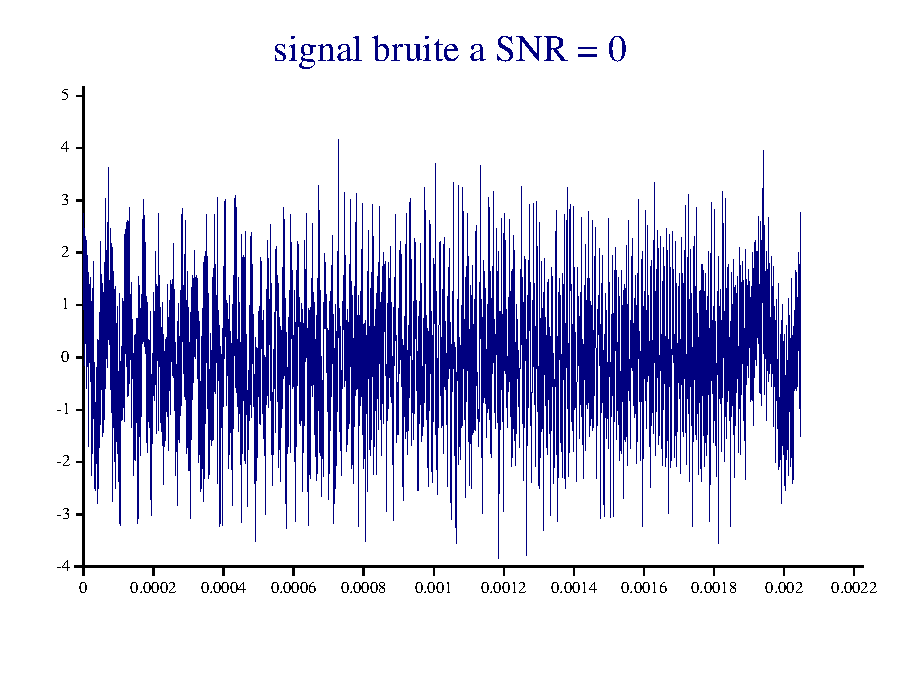
\includegraphics[width=0.9\linewidth]{frames/signal0.pdf}
			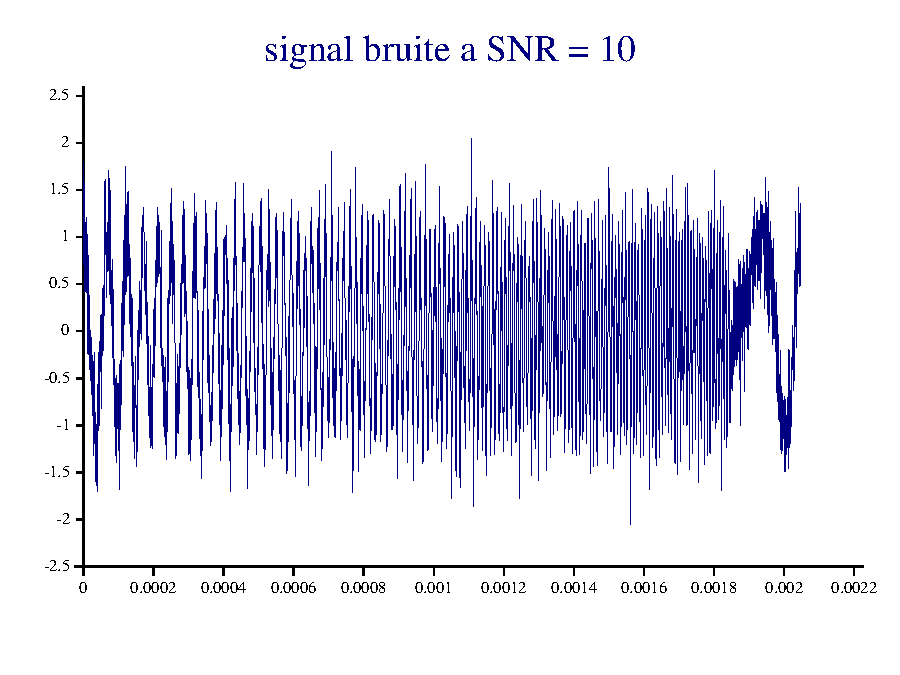
\includegraphics[width=0.9\linewidth]{frames/signal10.pdf}
		\end{columns}
	\end{frame}
	
	\begin{frame}
		\frametitle{demodulation}
		\begin{columns}
			\column{0.4\textwidth}
			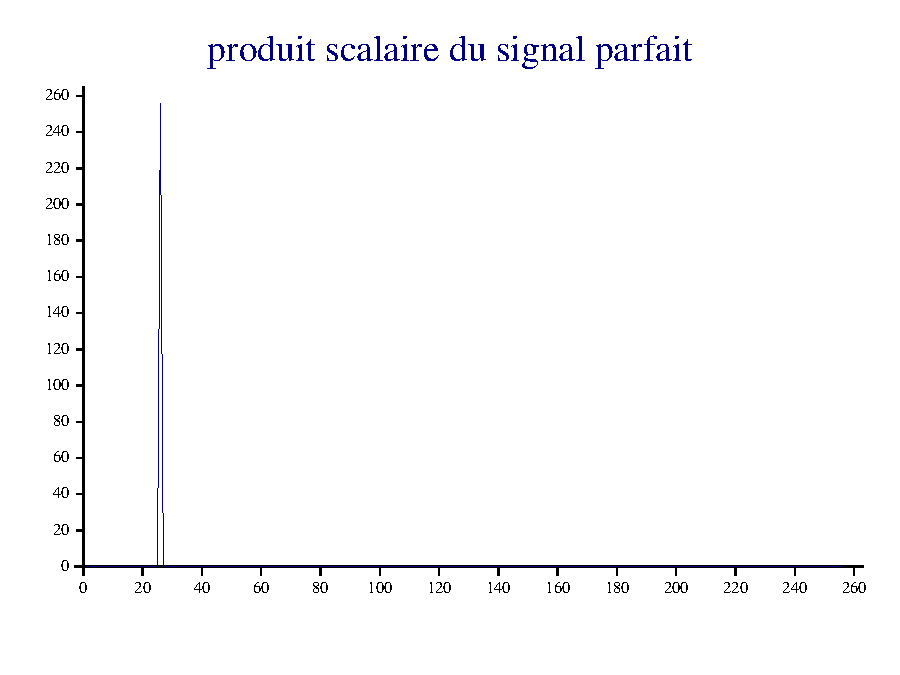
\includegraphics[width=\linewidth]{frames/perfectscalar.pdf}
			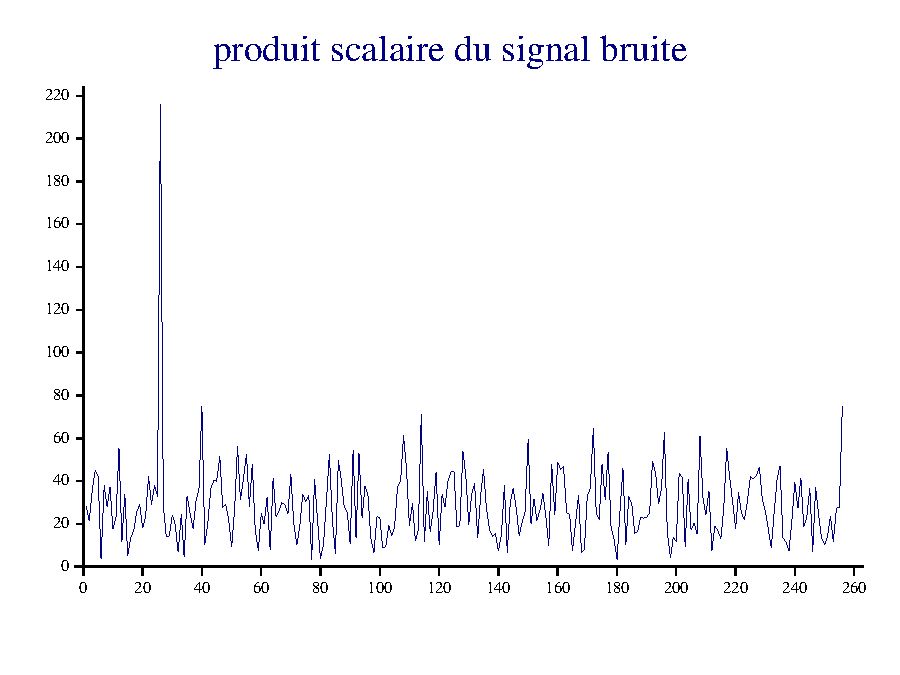
\includegraphics[width=\linewidth]{frames/noisyscalar.pdf}
			\column{0.5\textwidth}
			\begin{align*}
				\langle c_{s1}(t), c_{s2}(t)\rangle =
				\begin{cases}
					\|c_s(t)\|^2 & \text{si } s1 = s2\\
					0            & \text{si } s1 \neq s2\\
				\end{cases}
			\end{align*}
			$\Rightarrow s_1 = \underset{s_2}{\mathrm{argmax}}(\langle c_{s1}(t), c_{s2}(t)\rangle)$
		\end{columns}
	\end{frame}
	
	\begin{frame}
		\frametitle{transformation de Fourier}
		ce qui est équivalent à $s_1 = \underset{s_2}{\mathrm{argmax}}(\mathcal{F}(c_{s1}(t) c_{s2}^*(t)))$
		(annexe 3)\\
		\begin{columns}
			\column{0.5\linewidth}
			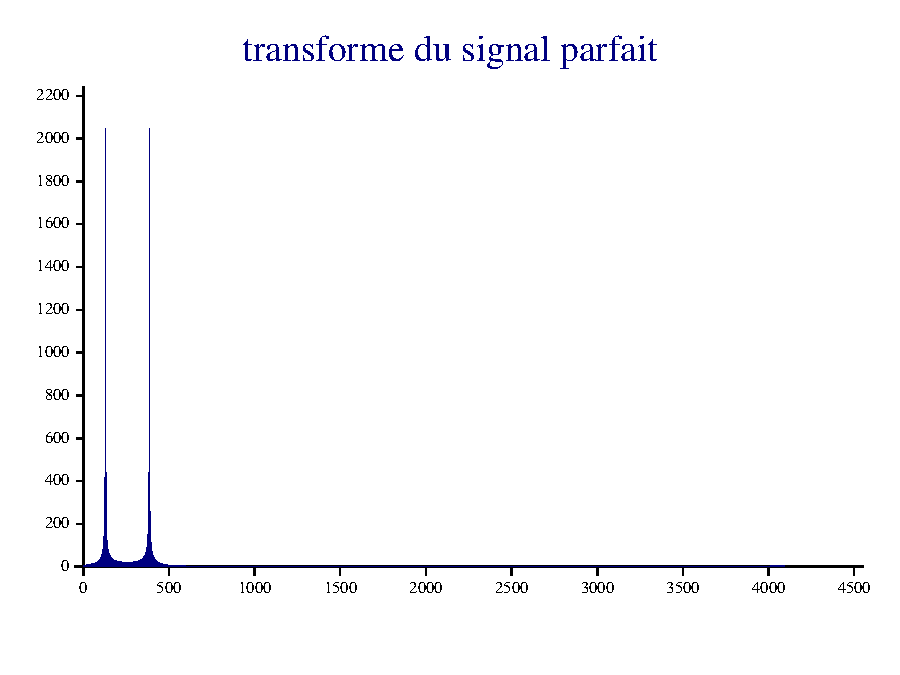
\includegraphics[width=\linewidth]{frames/perfectfft.pdf}
			\column{0.5\linewidth}
			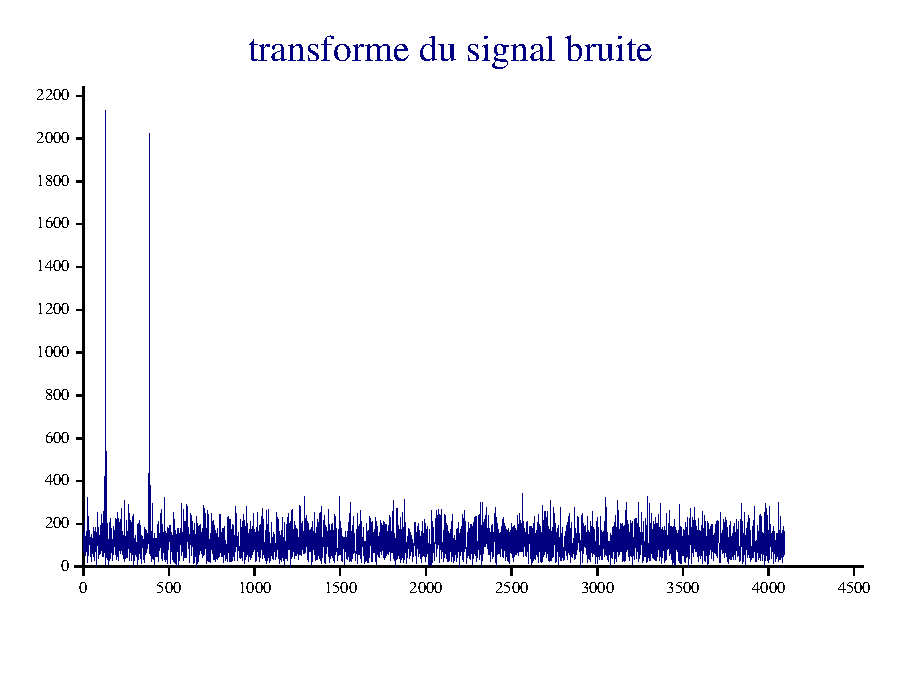
\includegraphics[width=\linewidth]{frames/noisyfft.pdf}
		\end{columns}
		Il y a un problème : deux sommets apparaissent, espacés d’une distance $B$
	\end{frame}
	
	\begin{frame}
		\frametitle{pourquoi ca ?}
		ici $SF = 8$ , $s = 128$ et le niveau de bruit $SNR = -10$dB
		\begin{columns}
			\column{0.6\linewidth}
			\centering
			\includegraphics[width=\linewidth]{frames/spectrogramC.png}
			spectrogram du signal parfait
			\includegraphics[width=\linewidth]{frames/spectrogramR.png}
			spectrogram du signal bruité
			\column{0.55\linewidth}
			\centering
			\includegraphics[width=\linewidth]{frames/spectrogramD.png}
			spectrogram du $c_0^*(t)$
			\includegraphics[width=\linewidth]{frames/spectrogramdemod.png}
			spectrogram du produit du $c_s$ et $c_0^*$
		\end{columns}
		
	\end{frame}
	
	\begin{frame}
		\frametitle{Comment résoudre ce problème ?}
		On peut utiliser une technique appelée undersampling, qui consiste à échantillonner le signal à une fréquence inférieure à celle recommandée par le théorème de Nyquist-Shannon.\\
		\centering
		\includegraphics[width=0.6\linewidth]{frames/undersampling.png}
	\end{frame}
	
	\begin{frame}
		\frametitle{Résultats d’undersampling}
		\begin{columns}
			\column{0.3\linewidth}
			\includegraphics[width=\linewidth]{frames/undersampledrizz.png}
			\column{0.5\linewidth}
			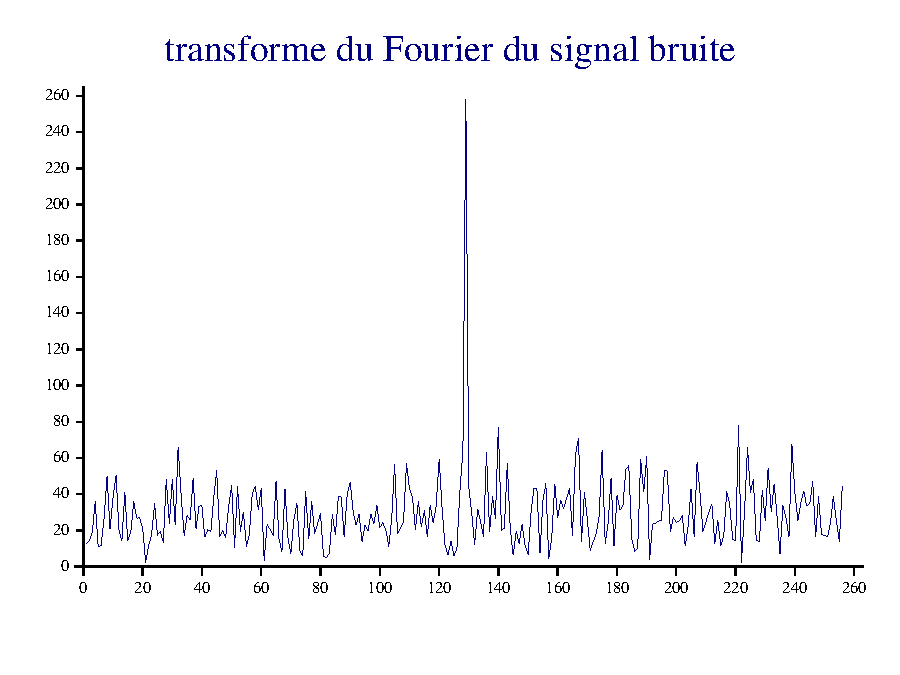
\includegraphics[width=\linewidth]{frames/noisyfftundersampled.pdf}
			\column{0.35\linewidth}
			d'abord on peut obtenir le symbole transmis par: $\displaystyle \hat{s} = \frac{2^{SF}}{B} \underset{p}{\mathrm{argmax}}\mathcal{F}(c_pc_0^*)$
		\end{columns}
	\end{frame}
	
	\begin{frame}
		\frametitle{performance théorique}
		\centering
		\begin{overpic}[width=0.9\linewidth]{frames/BERSNR.pdf}
			\put(25, 30){\tiny$SF = 16$}
			\put(35, 25){\tiny$SF = 15$}
			\put(44, 30){\tiny$SF = 14$}
			\put(53, 25){\tiny$SF = 13$}
			\put(62, 30){\tiny$SF = 12$}
			\put(71, 25){\tiny$SF = 11$}
			\put(80, 30){\tiny$SF = 10$}
			\put(89, 35){\tiny$SF = 9$}
			\put(90, 45){\tiny$SF = 8$}
			\put(99, 10){$SNR$}
			\put(00, 60){$BER$}
		\end{overpic}
	\end{frame}
	
	
	\begin{frame}
		\frametitle{le cas d'utilisation}
		\centering
		\begin{figure}[h]
			\includegraphics[width=\linewidth]{frames/usecase.png}
			\caption{cas d’utilisation du système}
		\end{figure}
	\end{frame}
	\begin{frame}
		\frametitle{diagrame de exigrences}
		\begin{figure}[h]
			\includegraphics[width=\linewidth]{frames/requirements.pdf}
			\caption{diagramme des exigences}
		\end{figure}
	\end{frame}

	\begin{frame}
		\frametitle{asservissement}
			\begin{figure}
				\centering
				\resizebox{\linewidth}{!}{
				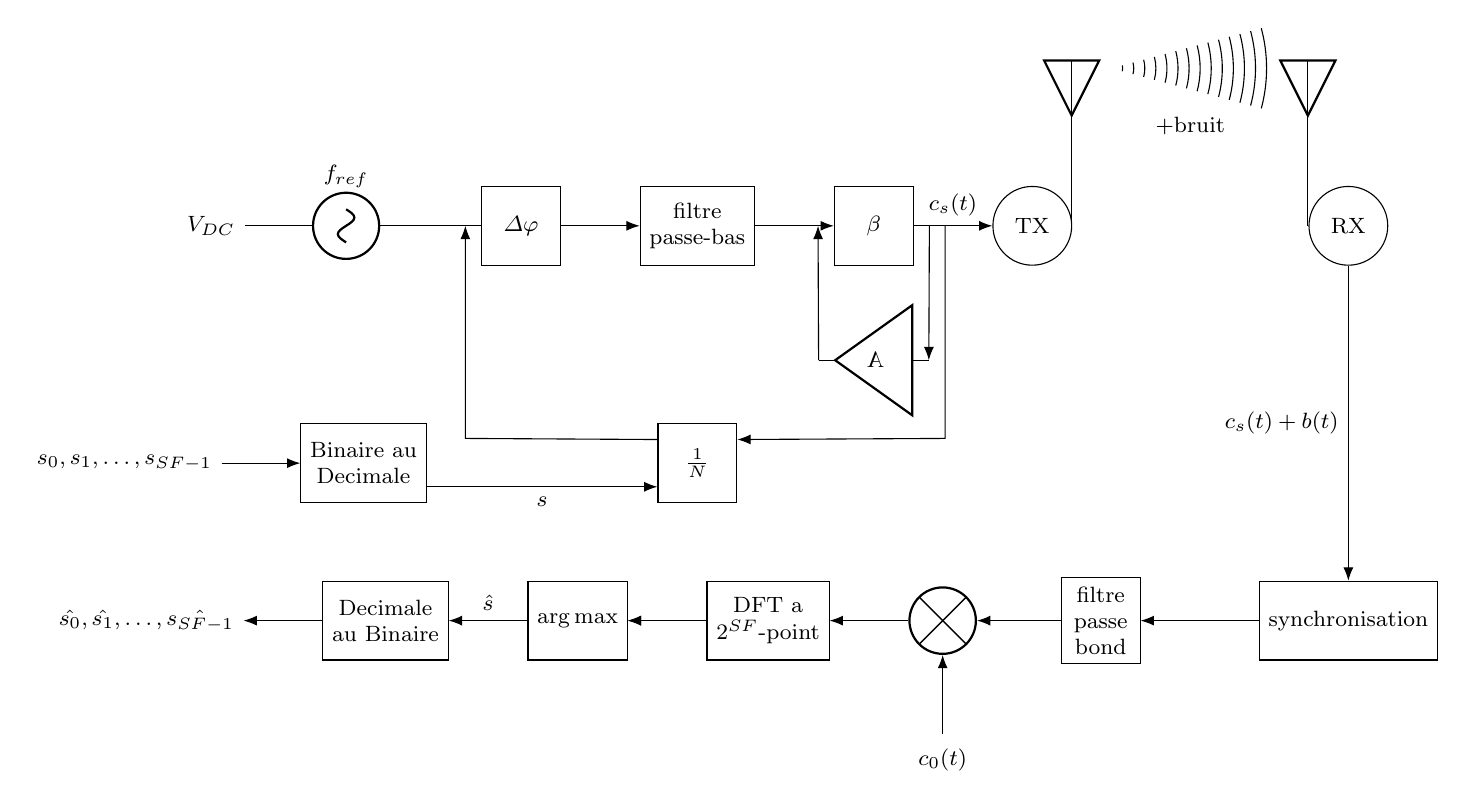
\begin{tikzpicture}[
					block/.style={draw, minimum height=1cm, minimum width=1cm, align=center},
					arrow/.style={->, >=Latex},
					smallblock/.style={draw, minimum height=1cm, minimum width=1.8cm},
					roundblock/.style={draw, circle, minimum size=1cm, inner sep=0pt, align=center},
					coord/.style={coordinate},
					font=\footnotesize
					]
					
					\node[block] (phasedef) {$\varDelta\varphi$};
					\node[block, right=1cm of phasedef] (loopfiltr) {filtre\\passe-bas};
					\node[block, right=1cm of loopfiltr] (vco) {$\beta$};
					\node[buffer,xscale=-1 ,below=0.5cm of vco] (amp) {A};
					\node[left=3cm of phasedef] (vin) {$V_{DC}$};
					\node[block, below=2cm of loopfiltr] (coef) {$\frac{1}{N}$};
					\draw(vin) to[sV, l=$f_{ref}$] (phasedef.west);
					\node[block, below=2cm of phasedef, xshift=-2cm] (binary2dec) {Binaire au\\Decimale};
					\node[left=of binary2dec] (inbits) {$s_0, s_1, \ldots, s_{SF-1}$};
					\node[roundblock, right=1cm of vco] (tx) {TX};
					\node[roundblock, right=3cm of tx] (rx) {RX};
					\node[antenna] at (tx.east) (ant1) {};

					\node[antenna] at (rx.west) (ant2) {};
					\node[block, below=4cm of rx] (sync) {synchronisation};
					\node[block, left=1.5cm of sync] (filtr) {filtre\\passe\\bond};
					\mixer{([xshift=-1.5cm]filtr.west)}{mixer};
					\node[block, left=1cm of mixer] (dft) {DFT a\\$2^{SF}$-point};
					\node[block, left=1cm of dft] (argmax) {$\argmax$};
					\node[block, left=1cm of argmax] (dec2binary) {Decimale\\au Binaire};
					\node[left=1cm of dec2binary] (outbits) {$\hat{s_0}, \hat{s_1}, \ldots, \hat{s_{SF-1}}$};
					
					% Connections
					\draw[arrow] (inbits) -- (binary2dec);
					\draw[arrow] (phasedef) -- (loopfiltr);
					\draw[arrow] ([shift={(0mm,-3mm)}]binary2dec.east) -- ([shift={(0mm,-3mm)}]coef.west) node[midway, below] {$s$};
					\draw[arrow] (loopfiltr) -- (vco);
					\draw[arrow] ([shift={(2mm,0cm)}]vco.east) -- (amp.west);
					\draw[arrow] ([shift={(0mm,3mm)}]coef.west) -- ([shift={(-2mm,-2.7cm)}]phasedef.west) -- ([shift={(-2mm,0cm)}]phasedef.west);
					\draw[arrow] ([shift={(4mm,0cm)}]vco.east) -- ([shift={(4mm,-2.7cm)}]vco.east) -- ([shift={(0mm,3mm)}]coef.east);
					\draw[arrow] (amp.east) -- ([shift={(-2mm,0cm)}]vco.west);
					\draw[arrow] (vco) -- (tx) node[midway, above] {$c_s(t)$};
					\draw[radiation] ([shift={(5mm,2cm)}]tx.east)-- node [below=5mm] {+bruit} ([shift={(-5mm,2cm)}]rx.west);
					\draw[arrow] (rx) -- (sync) node[midway, left] {$c_s(t)+b(t)$};
					\draw[arrow] (sync) -- (filtr);
					\draw[arrow] (filtr) -- (mixer);
					\draw[arrow] ([yshift=-1cm]mixer.south) -- (mixer) node[below=1.5cm] {$c_0(t)$};
					\draw[arrow] (mixer) -- (dft);
					\draw[arrow] (dft) -- (argmax);
					\draw[arrow] (argmax) -- (dec2binary) node[midway, above] {$\hat{s}$};
					\draw[arrow] (dft) -- (argmax);
					\draw[arrow] (dec2binary) -- (outbits);

				\end{tikzpicture}
				}
			\end{figure}
	\end{frame}

	\begin{frame}
		\frametitle{le block $\beta$}
		\begin{columns}
		\column{0.8\linewidth}
			\begin{overpic}[width=\linewidth]{frames/bode.png}
				\put(60, 43){\tiny 47nH}
				\put(82, 43){\tiny 5pF}
				\put(65,  9){\tiny 5pF}
				\put(83,  9){\tiny 7pF}
			\end{overpic}
		\column{0.3\linewidth}
			la pulsation de resonance est\\
			$\omega_0 \approx $ 2.56$\times10^9$rad/s \\ $\approx$ 410 MHz.\\~\\
			bien dans la bande ISM pour pouvoir diffuser sans avoir une licence.
		\end{columns}
	\end{frame}
	\begin{frame}
		\frametitle{circuit du VCO}
		\begin{columns}
			\column{0.3\linewidth}
				Les resultats de simulations:\\
				La consommation energitique\\$P_a \approx$ 16mW,\\~\\
				La distorsion harmonique totale $THD \approx$ 3.37\%.
			\column{0.8\linewidth}
				\includegraphics[width=\linewidth]{frames/vco.png}
		\end{columns}
	\end{frame}
	\begin{frame}
		\frametitle{frequence d'oscillation en fonction du voltage}
		\centering
		\includegraphics[width=0.8\linewidth]{frames/vcograph.png}
	\end{frame}
	\begin{frame}
		Le VCO consome 16 mW + ESP32 en mode 80 MHz 100mW.\\
		Totale 116mW quand le circuit est en operation.\\
		\centering
		\includegraphics[width=0.8\linewidth]{frames/batriyat.jpg}
	\end{frame}
	
	\begin{frame}
		\section{Conception et résultats expérimentaux d'un transmetteur}
		\frametitle{Conception expérimentale}
		\begin{columns}
			\column{0.3\linewidth}
			\includegraphics[width=\linewidth]{frames/pcblayout.png}
			\includegraphics[width=\linewidth]{frames/expe1.jpg}
			\column{0.3\linewidth}	
			\includegraphics[width=\linewidth]{frames/expe2.jpg}
			\column{0.3\linewidth}
			\includegraphics[width=\linewidth]{frames/expe3.jpg}
		\end{columns}
	\end{frame}

\begin{frame}
	\frametitle{Les logiciels utilisé pedant l'experience}
	\centering
	\begin{columns}
		\column{.5\linewidth}
		\includegraphics[width=.7\linewidth]{frames/nuevayol.jpg}
		\column{.5\linewidth}
		\includegraphics[width=.7\linewidth]{frames/callmeundone.jpg}
	\end{columns}
	\includegraphics[width=.9\linewidth]{frames/opheliawannabe.png}
\end{frame}

	\begin{frame}
		\centering
		\begin{columns}
		\column{.5\linewidth}
		\includegraphics[width=1.1\linewidth]{frames/tagant1.jpg}
		\column{.5\linewidth}
		\includegraphics[width=\linewidth]{frames/tagant2.jpg}
		\end{columns}
	\end{frame}
	\begin{frame}
		\frametitle{Résultats expérimentaux}
		\centering
		\includegraphics[height=0.7\linewidth]{frames/tagant3.png}
	\end{frame}

	\begin{frame}
		\section{Conclusion}
		\centering
		Conclusion
	\end{frame}

	\section{Les annexes}
	
	\begin{frame}
		\frametitle{annexe 1: Dérivation de l'expression de la fréquence}
		derivation d'expression de $f_s(t)$
		on a $\displaystyle a = \frac{B}{T}$ et $b = \frac{s}{2^{SF}}B$
		$\displaystyle\Rightarrow f_s(t) = (\frac{t}{T}B + \frac{s}{2^{SF}}B)_{mod B}$
		$ = (B (\frac{t}{T} + \frac{s}{2^{SF}}))_{mod B} =  B ((\frac{t}{T} + \frac{s}{2^{SF}})_{mod 1})$
		$ = B (\frac{1}{2^{SF}}(2^{SF}\frac{t}{T} + s)_{mod 1}) = (s + \dfrac{t}{T}2^{SF})_{mod  2^{SF}} \dfrac{B}{2^{SF}}$
	\end{frame}
	
	\begin{frame}
		\frametitle{annexe 2: Démonstration de l’orthogonalité}
		soit $F$ un $\mathbb{C}^\mathbb{R}$ espace vecteuriel definee par $F = Vect((c_s(t))_{0\leq s<2^{SF}})$.\\
		soit $(p, q) \in \textlbrackdbl0, 2^{SF}\textlbrackdbl^2$ tel que $p\geq q$, sans perder de generalite.\\
		soit l'application $\displaystyle\langle P,Q\rangle = \int_{0}^{T} P(t)Q^*(t)dt$, avec $Q^*$ est le conjuguee complex du $Q$, un produit scalaire dans $\mathbb{C}^\mathbb{R}$.\\
		alors $\displaystyle\langle c_{s=p}, c_{s=q}\rangle = \int_{0}^{T} c_p(t)c_q^*(t)dt = \int_{0}^{t_f} \exp(j2\pi((\frac{p}{2^{SF}})Bt+\frac{Bt^2}{2T}-(\frac{q}{2^{SF}})Bt - \frac{Bt^2}{2T}))dt + \int_{t_f}^{t_f'} \exp(j2\pi((\frac{p}{2^{SF}})Bt+\frac{Bt^2}{2T} - (\frac{q}{2^{SF}})Bt - \frac{Bt^2}{2T} + Bt))dt + \int_{t_f'}^{T}\exp(j2\pi((\frac{p}{2^{SF}})Bt+\frac{Bt^2}{2T} - Bt - (\frac{q}{2^{SF}})Bt - \frac{Bt^2}{2T} + Bt))dt = $
		
	\end{frame}
	\begin{frame}
		\frametitle{annexe 2 (suite)}
		$\displaystyle\int_{0}^{t_f} \exp(j2\pi(\frac{p-q}{2^{SF}}Bt))dt + \int_{t_f}^{t_f'}\exp(j2\pi((\frac{p-q}{2^{SF}} + 1)Bt))dt + \int_{t_f'}^{T}\exp(j2\pi(\frac{p-q}{2^{SF}})Bt)dt = \frac{2^{SF}}{j2\pi(p-q)B}(\exp(j2\pi \frac{p-q}{2^{SF}}Bt_f')-1) + \frac{2^{SF}}{j2\pi(p-q+2^{SF})B}(\exp(j2\pi \frac{p-q+2^{SF}}{2^{SF}}Bt_f)-\exp(j2\pi \frac{p-q+2^{SF}}{2^{SF}}Bt_f')) + \frac{2^{SF}}{j2\pi(p-q)B}(1 - \exp(j2\pi \frac{p-q}{2^{SF}}Bt_f))$\\
		\begin{align*}
			\Rightarrow \displaystyle\langle c_{p}, c_{q}\rangle
			\begin{cases}
				(t_f = t_f') = 0 & p = q\\
				\neq 0 & p \neq q\\
			\end{cases}
		\end{align*}
		donc la bases $F = Vect((c_s(t))_{0\leq s<2^{SF}})$ de $F$ est orthogonale.
	\end{frame}
	
	
	\begin{frame}
		\frametitle{annexe 3: Étude théorique d’une transformation de Fourier}
		soit $p \in \textlbrackdbl0, 2^{SF}\textlbrackdbl$\\
		\begin{align*}
			c_p c_{s=0}^* =
			\begin{cases}
				\exp ({j 2 \pi ({ ({\frac {p}{2^{SF}}}) Bt + \frac {B}{2T} t^{2}}) }) \exp ({-j2 \pi ({\frac {B}{2T} t^{2}})}) & 0 \leq t < t_f \\
				\exp ({j 2 \pi ({ ({\frac {p}{2^{SF}} - 1}) Bt + \frac {B}{2T} t^{2} }) }) \exp ({-j2 \pi ({\frac {B}{2T} t^{2}})}) & t_f \leq t < T
			\end{cases}
		\end{align*}
		\begin{align*}
			= \begin{cases}
				\exp(j2\pi((\frac{p}{2^{SF}})Bt)) & 0 \leq t < t_f \\
				\exp(j2\pi((\frac{p}{2^{SF}})Bt - Bt)) & t_f \leq t < T
			\end{cases}
		\end{align*}
		$\Rightarrow c_pc_0(t_f \leq t < T) = c_pc_0(0\leq t < t_f) \exp(-j2\pi Bt)$\\
		$\Rightarrow \argmax\mathcal{F}(c_pc_0(0\leq t < t_f)) = p \dfrac{B}{2^{SF}}$ et $\argmax\mathcal{F}(c_pc_0(t_f \leq t < T)) = p \dfrac{B}{2^{SF}} - B$
	\end{frame}
	
	\begin{frame}
		\frametitle{annexe 4: Le code pour générer les courbes}
		\centering
		\begin{columns}
			\column{0.5\linewidth}
			\includegraphics[width=\linewidth]{frames/code1.png}
			\column{0.5\linewidth}
			\includegraphics[width=\linewidth]{frames/code2.png}
		\end{columns}
	\end{frame}
	
	\begin{frame}
		\frametitle{annexe 4: suite}
		\centering
		\begin{columns}
			\column{0.6\linewidth}
			\includegraphics[width=\linewidth]{frames/code3.png}
			\column{0.55\linewidth}
			\includegraphics[width=\linewidth]{frames/code4.png}
		\end{columns}
	\end{frame}
	
	\begin{frame}
		\frametitle{annexe 5: Le code pour realiser l'experience (ESP32)}
		\begin{columns}
			\column{0.5\linewidth}
			\includegraphics[width=1.1\linewidth]{frames/alreadywokespreadajokestareatfolkswhenproperlyprovokemirorbroke.png}
			\column{0.5\linewidth}
			\includegraphics[width=1.1\linewidth]{frames/hereshareastrawberrymorninggoneamoreimportantspawningtorninpoormenswrnin.png}
		\end{columns}
	\end{frame}
	\begin{frame}
		\frametitle{annexe 5: Le code pour realiser l'experience (GNU Radio)}
		\centering
		\includegraphics[width=\linewidth]{frames/cornersendswitchingpositionsoditionningmortitionssawitinvisionignoringprison.pdf}
	\end{frame}
	
	
\end{document}